\documentclass[tikz,border=10pt]{standalone}
\usepackage{amssymb}
\usetikzlibrary{shapes.geometric,fit}

\begin{document}
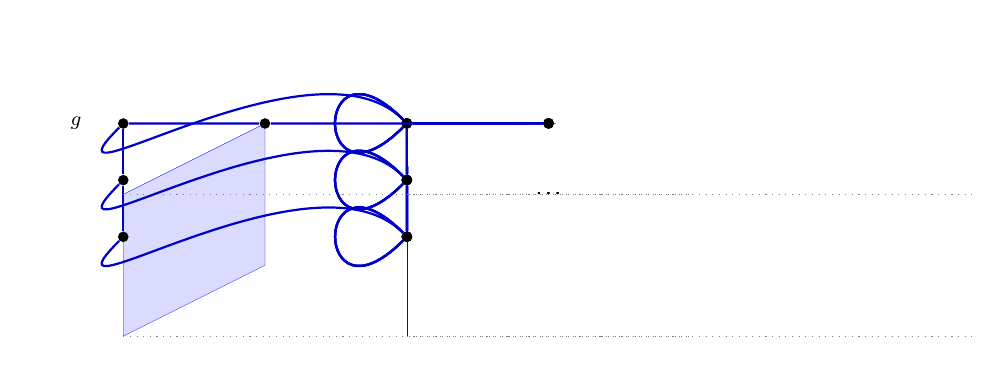
\begin{tikzpicture}[scale=1.2, every node/.style={scale=0.9}]

% Define styles for nodes and edges
\tikzset{
    dot/.style={circle, fill=black, inner sep=1.5pt},
    edge/.style={thick, draw=blue!80!black},
    layer/.style={draw=blue, fill=blue!20, fill opacity=0.7, ultra thin},
    label/.style={font=\footnotesize, anchor=center},
}

% Define coordinates for layers and nodes
\def\layersep{1.5}
\def\nodesepr{0.6}
\def\nodepos{(0,0)}

% Draw the layers and nodes
\foreach \i [count=\j from 0] in {1,...,6} {
    % Draw the parallelogram for each layer
    \ifnum\i=1
        \coordinate (A\i) at (0,\i*\layersep);
        \coordinate (B\i) at (\layersep,\i*\layersep+\layersep/2);
        \coordinate (C\i) at (\layersep,\i*\layersep-\layersep/2);
        \coordinate (D\i) at (0,\i*\layersep-\layersep);
    \else
        \coordinate (A\i) at (A\j -| 2*\layersep, \i*\layersep);
        \coordinate (B\i) at (B\j -| 2*\layersep, \i*\layersep+\layersep/2);
        \coordinate (C\i) at (C\j -| 2*\layersep, \i*\layersep-\layersep/2);
        \coordinate (D\i) at (D\j -| 2*\layersep, \i*\layersep-\layersep);
    \fi
    
    % Draw the parallelogram
    \draw[layer] (A\i) -- (B\i) -- (C\i) -- (D\i) -- cycle;
    
    % Add nodes inside the parallelogram
    \node[dot] (n\i1) at (A\i |- B\i) {};
    \node[dot] (n\i2) at ([yshift=-\nodesepr cm] n\i1) {};
    \node[dot] (n\i3) at ([yshift=-\nodesepr cm] n\i2) {};
    \node[dot] (n\i4) at ([xshift=\layersep cm] n\i1) {};
    
    % Connect nodes within the same layer
    \draw[edge] (n\i1) -- (n\i2);
    \draw[edge] (n\i2) -- (n\i3);
    \draw[edge] (n\i1) -- (n\i4);
    
    % Add label "g" near the first node in the first layer
    \ifnum\i=1
        \node[label] at ([xshift=-0.5cm] n\i1) {$g$};
    \fi
}

% Add ellipses between layers
\foreach \i in {2,...,5} {
    \node[label] at ([xshift=\layersep cm] A\i) {$\cdots$};
}

% Add connections between layers
\draw[edge] (n11) .. controls +(-1,-1) and +(-1,1) .. (n21);
\draw[edge] (n12) .. controls +(-1,-1) and +(-1,1) .. (n22);
\draw[edge] (n13) .. controls +(-1,-1) and +(-1,1) .. (n23);
\draw[edge] (n14) -- (n24);

\draw[edge] (n21) .. controls +(-1,-1) and +(-1,1) .. (n31);
\draw[edge] (n22) .. controls +(-1,-1) and +(-1,1) .. (n32);
\draw[edge] (n23) .. controls +(-1,-1) and +(-1,1) .. (n33);
\draw[edge] (n24) -- (n34);

\draw[edge] (n31) .. controls +(-1,-1) and +(-1,1) .. (n41);
\draw[edge] (n32) .. controls +(-1,-1) and +(-1,1) .. (n42);
\draw[edge] (n33) .. controls +(-1,-1) and +(-1,1) .. (n43);
\draw[edge] (n34) -- (n44);

\draw[edge] (n41) .. controls +(-1,-1) and +(-1,1) .. (n51);
\draw[edge] (n42) .. controls +(-1,-1) and +(-1,1) .. (n52);
\draw[edge] (n43) .. controls +(-1,-1) and +(-1,1) .. (n53);
\draw[edge] (n44) -- (n54);

\draw[edge] (n51) .. controls +(-1,-1) and +(-1,1) .. (n61);
\draw[edge] (n52) .. controls +(-1,-1) and +(-1,1) .. (n62);
\draw[edge] (n53) .. controls +(-1,-1) and +(-1,1) .. (n63);
\draw[edge] (n54) -- (n64);

% Add dotted lines separating layers
\foreach \i in {1,...,5} {
    \draw[dotted, gray] (A\i) -- ++(4*\layersep,0);
    \draw[dotted, gray] (D\i) -- ++(4*\layersep,0);
}

\end{tikzpicture}
\end{document}